\documentclass[10pt,conference,letterpaper]{IEEEtran}

\usepackage{cite}
\usepackage{amsmath,amssymb}
\usepackage{booktabs}
\usepackage{graphicx}
\usepackage{textcomp}
\usepackage{xcolor}
\usepackage{url}
\usepackage{tikz}
\usetikzlibrary{arrows.meta,positioning,fit}

\def\BibTeX{{\rm B\kern-.05em{\sc i\kern-.025em b}\kern-.08em
    T\kern-.1667em\lower.7ex\hbox{E}\kern-.125emX}}

\graphicspath{{./}}
\newcommand{\system}{cuSZp-KV}
% BEGIN GENERATED: results_macros
% Generated from canonical experiment JSON; do not edit this block.
\newcommand{\ConcurrencyHandlerReductionPct}{25.5\%}
\newcommand{\ConcurrencyThroughputGainPct}{20.6\%}
\newcommand{\ArrivalAchievedGainPct}{17.7\%}
\newcommand{\ArrivalTTFTPReductionPct}{38.4\%}
\newcommand{\SmallHandlerReductionPct}{25.5\%}
% END GENERATED: results_macros

% INFOCOM 2027 uses double-blind review. Keep this true for submission and
% change it to \anonymousfalse only for the accepted camera-ready manuscript.
\newif\ifanonymous
\anonymoustrue

\begin{document}

\title{Crossing the PCIe Break-Even Point with GPU-Native
Error-Bounded KV-Cache Transfers}

\ifanonymous
\author{}
\else
\author{
\IEEEauthorblockN{Zirui Kong}
\IEEEauthorblockA{\textit{Department of Computing}\\
\textit{The Hong Kong Polytechnic University}\\
Hong Kong, China\\
jerryhongkong.kong@connect.polyu.hk}
\and
\IEEEauthorblockN{Jiayi Li}
\IEEEauthorblockA{\textit{International School}\\
\textit{Beijing University of Posts and}\\
\textit{Telecommunications}\\
Beijing, China\\
lijiayi2022@bupt.edu.cn}
\and
\IEEEauthorblockN{Zhaorui Zhang}
\IEEEauthorblockA{\textit{Department of Computing}\\
\textit{The Hong Kong Polytechnic University}\\
Hong Kong, China\\
zhaorui.zhang@polyu.edu.hk}
}
\fi

\maketitle

\begin{abstract}
Long-context large language model serving may move key--value caches between graphics processing unit memory and host memory, making Peripheral Component Interconnect Express transfer a critical latency component. Compression helps only when the saved transfer time exceeds encoding, metadata, synchronization, and decoding overhead. We present \system{}, a vLLM-compatible cache-transfer path that combines device-side error-bounded compression, event-ordered background offload, reusable device workspaces, packed pinned-memory transfers, and batched bfloat16 restoration. On an RTX 5080, five interleaved trials with Qwen2.5-1.5B show that, at concurrency eight, \system{} reduces combined offload-and-restore handler time by \ConcurrencyHandlerReductionPct{} and increases initial request throughput by \ConcurrencyThroughputGainPct{} relative to a matched raw path. At an overloaded arrival rate of six requests per second, it increases achieved throughput by \ArrivalAchievedGainPct{} and reduces the 95th-percentile time to first token by \ArrivalTTFTPReductionPct{}, although neither path sustains the offered load. A second Qwen2.5-0.5B workload matches raw output under predefined quality gates and reduces handler time by \SmallHandlerReductionPct{}. Across eight models, cuSZp has lower handler time than matched 8-bit quantization, Zstandard, and LZ4 paths, while gains over raw transfer remain workload dependent. A two-trial mixed-bound pilot preserves quality but remains slower than the optimized fixed-bound path, identifying adaptation overhead as future work.
\end{abstract}

\begin{IEEEkeywords}
large language model serving, key--value cache offloading, host--device transfer,
device-side compression, error-bounded compression
\end{IEEEkeywords}

\section{Introduction}
\label{sec:introduction}

Paged KV-cache management makes high-throughput LLM serving possible by
allocating attention state at block granularity instead of reserving a
contiguous worst-case buffer for every request~\cite{kwon2023pagedattention}.
When GPU memory becomes scarce, however, serving engines must preempt requests
and move cache blocks to host memory.  Long contexts and concurrent requests
make this transient state large, while every restored byte must cross a
CPU--GPU interconnect whose bandwidth is far below on-device memory
bandwidth~\cite{li2020gpuinterconnect}.  Disaggregated systems make KV-cache
placement and transfer first-class scheduling concerns~\cite{qin2025mooncake};
the same data-movement problem appears within a single server when DRAM extends
the GPU memory tier.

Compression appears to offer a direct solution: transmitting $S/\rho$ bytes
instead of $S$ bytes should reduce transfer time by the compression ratio
$\rho$.  In practice, this argument is incomplete.  A compressed transfer also
pays for range reduction, encoding, variable-length metadata, device and host
allocation, synchronization, decoding, and placement into final KV pages.  A
prototype can therefore report an attractive compression ratio while remaining
slower than an optimized raw copy.  This was the central engineering obstacle
in our project.

We present \system{}, a GPU-native, error-bounded KV-cache transfer path for
vLLM.  The system is loaded through vLLM V1's native offloading connector
without changing the installed vLLM package, model, or scheduler.  It orders
background offload after a producer-stream event, packs variable-length outputs
into reusable device slabs and pinned host storage, and decodes a restore batch
directly into BF16 KV pages.  The production configuration uses fixed cuSZp with
a conservative relative bound of $10^{-5}$.  A model-calibrated adaptive
controller is implemented, but is deliberately reported as an ablation because
it does not yet beat the fixed path.

Our evaluation is designed around the break-even question rather than
compression ratio alone.  We compare against a matched asynchronous raw path,
use five interleaved trials, preserve fixed wall-clock arrivals in an open-loop
driver, pool request samples only for descriptive tail percentiles, and use
paired trial-level confidence intervals for performance claims.  We evaluate
eight locally cached models and common compressed baselines, and retain
workloads that favor raw or fail a quality gate.

This paper makes four contributions:

\begin{itemize}
  \item We build a transparent vLLM compress--transfer--decompress path whose
  raw and compressed modes share pinned storage, batching, destination pages,
  scheduling class, and timing boundaries.
  \item We remove practical break-even blockers through persistent GPU
  workspaces, packed D2H/H2D slabs, event-ordered background offload, and a batched
  fixed-cuSZp decoder that writes BF16 values directly to final KV pages.
  \item We introduce a reproducible evaluation protocol combining real
  simultaneous bursts, fixed-rate open-loop arrivals, pooled P95/P99 and SLO
  metrics, strict raw-relative quality gates, and paired five-trial intervals.
  \item We demonstrate quality-safe raw break-even on two Qwen2.5 models and
  compare five transfer methods across eight models, while explicitly
  documenting negative model and adaptive-controller results.
\end{itemize}

\section{Background and Related Work}
\label{sec:related}

\subsection{KV-Cache Memory and Offloading}

Autoregressive attention reuses the keys and values of all preceding tokens.
The KV cache consequently grows with sequence length, layer count, hidden
dimension, and active request count.  vLLM's PagedAttention reduces
fragmentation and enables block-granular sharing and preemption
\cite{kwon2023pagedattention}, but preempted state still needs a backing tier.
FlexGen jointly schedules GPU, CPU, and storage placement for
memory-constrained inference and also considers low-bit attention-cache
representations~\cite{sheng2023flexgen}.  InfiniGen reduces host-fetch traffic
by speculating which KV entries will be useful~\cite{lee2024infinigen}.
MOONCAKE extends KV-cache placement across DRAM, SSD, and networked serving
resources~\cite{qin2025mooncake}.  These systems motivate our focus on the
local PCIe data plane: \system{} preserves vLLM's cache and scheduling semantics
and changes the representation used while blocks are in transit and in host
storage.

\subsection{KV-Cache Reduction}

KV-cache reduction spans eviction, quantization, and learned or structured
encoding.  $H_2O$ retains attention heavy hitters and evicts less important
tokens~\cite{zhang2023h2o}.  KIVI uses asymmetric 2-bit quantization to reduce
resident KV memory and increase feasible batch size~\cite{liu2024kivi}.
CacheGen encodes reusable KV caches for network streaming and adapts coding
levels to bandwidth~\cite{liu2024cachegen}.  Our target is different but
complementary: we compress pages selected by an existing vLLM cache manager,
optimize the single-node GPU--CPU transfer critical path, and compare with the
raw path under identical asynchronous storage and restore machinery.

\subsection{GPU Error-Bounded Compression}

cuSZp is a GPU-oriented error-bounded lossy compressor designed for high
end-to-end throughput on floating-point scientific data
\cite{huang2023cuszp}.  KV tensors differ from its original datasets in shape,
precision, lifetime, and quality semantics.  \system{} contributes the serving
integration: per-page relative-bound conversion, variable-length host metadata,
BF16 direct restore, raw fallback, and request-level quality validation.  We do
not claim a new codec or bitstream.

\section{Break-Even Model}
\label{sec:model}

Let $S$ be the raw bytes moved for a cache-transfer event, $B$ the effective
PCIe bandwidth, and $\rho$ the compression ratio.  A simplified raw path is
\begin{equation}
T_{\mathrm{raw}} = \tau_{\mathrm{raw}} + \frac{S}{B},
\end{equation}
where $\tau_{\mathrm{raw}}$ captures launch, bookkeeping, and placement
overheads.  The compressed path is
\begin{equation}
T_{\mathrm{cmp}} =
C(S,\epsilon) + \tau_{\mathrm{cmp}} + \frac{S}{\rho B}
+ D(S,\epsilon),
\end{equation}
where $C$ and $D$ are compression and decompression costs at error bound
$\epsilon$.  Compression wins only if
\begin{equation}
C + D + (\tau_{\mathrm{cmp}}-\tau_{\mathrm{raw}})
< \frac{S}{B}\left(1-\frac{1}{\rho}\right).
\label{eq:breakeven}
\end{equation}
Equation~\eqref{eq:breakeven} explains why fewer bytes do not guarantee lower
latency.  It also motivates three design rules: remove fixed per-event costs,
batch payloads before crossing PCIe, and retain raw as a valid action when the
measured operating point is below break-even.

\section{System Design}
\label{sec:design}

\begin{figure*}[t]
\centering
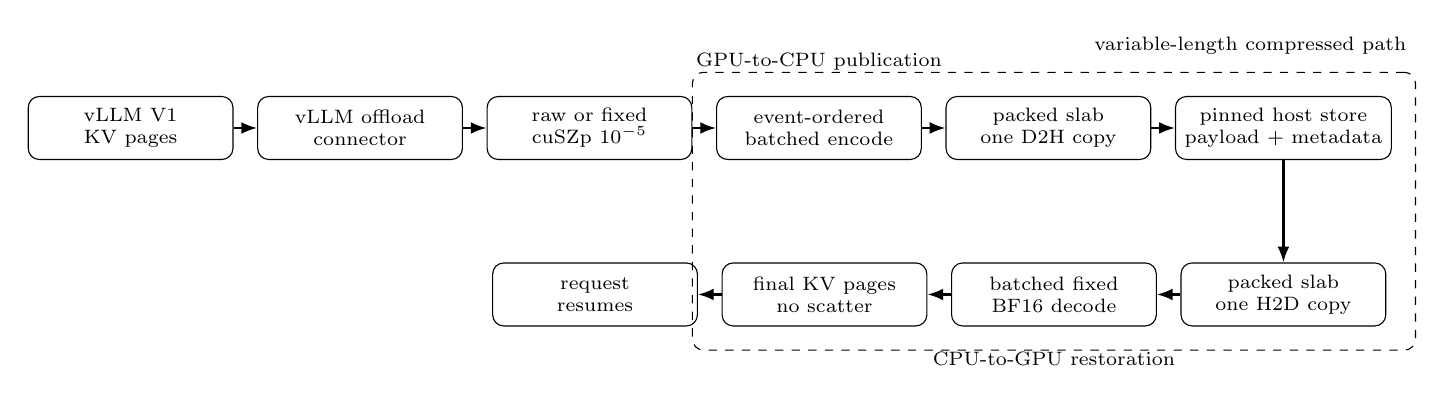
\begin{tikzpicture}[
  node distance=3mm and 3mm,
  box/.style={draw,rounded corners,align=center,minimum height=8mm,
              minimum width=24mm,font=\scriptsize},
  wide/.style={box,minimum width=26mm},
  arrow/.style={-{Latex[length=2mm]},thick},
  note/.style={font=\scriptsize,align=center}
]
\node[wide] (cache) {vLLM V1\\KV pages};
\node[wide,right=of cache] (patch) {vLLM offload\\connector};
\node[wide,right=of patch] (policy) {raw or fixed\\cuSZp $10^{-5}$};
\node[wide,right=of policy] (compress) {event-ordered\\batched encode};
\node[wide,right=of compress] (d2h) {packed slab\\one D2H copy};
\node[wide,right=of d2h] (host) {pinned host store\\payload + metadata};

\node[wide,below=13mm of host] (h2d) {packed slab\\one H2D copy};
\node[wide,left=of h2d] (decode) {batched fixed\\BF16 decode};
\node[wide,left=of decode] (pages) {final KV pages\\no scatter};
\node[wide,left=of pages] (resume) {request\\resumes};

\draw[arrow] (cache) -- (patch);
\draw[arrow] (patch) -- (policy);
\draw[arrow] (policy) -- (compress);
\draw[arrow] (compress) -- (d2h);
\draw[arrow] (d2h) -- (host);
\draw[arrow] (host) -- (h2d);
\draw[arrow] (h2d) -- (decode);
\draw[arrow] (decode) -- (pages);
\draw[arrow] (pages) -- (resume);

\node[note,above=2mm of compress] {GPU-to-CPU publication};
\node[note,below=2mm of decode] {CPU-to-GPU restoration};
\node[draw,dashed,rounded corners,fit=(compress)(d2h)(host)(h2d)(decode),
      inner sep=3mm] (compressedpath) {};
\node[note,anchor=south east]
      at ([yshift=1mm]compressedpath.north east)
      {variable-length compressed path};
\end{tikzpicture}
\caption{\system{} data path.  Raw mode shares the connector, pinned store,
batching, final destinations, and measurement boundaries, but bypasses codec
kernels and compressed metadata.}
\label{fig:architecture}
\end{figure*}

\subsection{Transparent Cache-Engine Interposition}

vLLM V1's native \texttt{OffloadingConnector} loads our
\texttt{CompressedCPUOffloadingSpec} through \texttt{spec\_module\_path}; no
Python monkey-patching or modification of the installed vLLM package is used.
The model, PagedAttention kernels, scheduler, and block identifiers remain
unchanged.  The connector maps each host-resident entry to its codec, original
shape, compressed length, destination page, and actual absolute error bound.
Unsupported fixed-fast-path layouts fall back to the generic bundle path; an
encoded payload that would expand falls back to the same raw representation
used by the matched baseline.

The C++/PyBind11 extension obtains the current PyTorch CUDA stream in the thread
that invokes each native operation.  For GPU-to-CPU offload, the connector first
records an event on vLLM's producer stream; a single background worker waits for
that event and then runs cuSZp on its own default CUDA stream.  This explicit
handoff is required because the tested cuSZp path is not reliable on a
non-default worker stream.  Publication synchronizes the producing stream before
making pinned-host slices visible.  Restore enqueues H2D copies and decoding on
the restore thread's current stream.  This is not a synchronization-free path:
it uses scoped event and stream synchronization, while the normal unprofiled
path avoids an unconditional device-wide barrier.

\subsection{Packed Publication and Restore}

Variable compressed sizes make per-page host allocation and copying expensive.
The GPU-to-CPU path reuses grow-only compression and packing workspaces where the
fixed fast path applies, computes payload offsets, concatenates the outputs into
one device slab, allocates a pinned host slab for the publication, and exposes
its slices after one scoped stream synchronization.  The host dictionary stores
those slices and reconstruction metadata; it does not copy the payload through
pageable Python buffers.

On restore, compatible pages are packed into one pinned-host slab and transferred
with one H2D copy.  The fixed-mode CUDA decoder consumes the packed metadata and
writes BF16 pairs directly into their final KV-page destinations.  It avoids an
intermediate FP32 output and a later GPU scatter.  The raw baseline likewise
uses pinned slabs and copies directly into final pages, making it a strong
break-even baseline rather than vLLM's unoptimized stock swap code.

\subsection{Error Bounds and Adaptive Extension}

cuSZp consumes an absolute bound, while KV activation ranges vary by page.  For
a configured relative bound $\epsilon_{\mathrm{rel}}$, the wrapper computes
\begin{equation}
\epsilon_{\mathrm{abs}} =
\epsilon_{\mathrm{rel}}\max(\max(T)-\min(T),10^{-6})
\end{equation}
with a CUDA reduction and stores the resulting scalar beside the bitstream.
The main system uses $\epsilon_{\mathrm{rel}}=10^{-5}$ because the registered
multi-prompt quality suite rejects uniform looser bounds.

The implementation also contains an optional cost-aware restore model that can
select raw fallback versus cuSZp using measured ratio and decoder throughput,
plus a pressure controller, model-specific per-layer safety caps, and cuSZp's
existing plain, fixed, or outlier mode.  Offline multi-prompt sweeps
conservatively merge per-layer quality constraints.  The formal adaptive pilot
uses fixed cuSZp mode and has the cost-aware option disabled; it therefore tests
the calibrated mixed-bound pressure mechanism rather than cost-model-based raw
selection.  Section~\ref{sec:adaptive} reports this quality-safe mechanism
separately because it is slower than the uniform fixed path.
\section{Evaluation Methodology}
\label{sec:methodology}

\subsection{Platform}

Experiments run under Ubuntu 24.04 on WSL2 with an Intel Core Ultra 7 265KF
(20 cores), 32~GB host memory, and an NVIDIA GeForce RTX 5080 with 16~GB
GDDR7.  The software stack uses Python 3.12.3, PyTorch 2.11.0 with CUDA 13.0,
Transformers 5.12.1, and vLLM 0.23.0.  The cuSZp extension is built from its
CUDA 12.0-compatible source with PTX enabled for the GPU.  vLLM uses its V1
model runner because UVA is reported unavailable in the tested WSL
configuration; every method records and shares this setting.

\subsection{Methods and Workloads}

We compare five data paths:

\begin{itemize}
  \item \textbf{Raw}: pinned asynchronous D2H/H2D slabs with direct final-page
  placement and no compression.
  \item \textbf{cuSZp}: the optimized fixed path at relative bound $10^{-5}$.
  \item \textbf{INT8}: an asynchronous 8-bit quantization/dequantization path.
  \item \textbf{Zstd and LZ4}: CPU compressed paths using the same host-store
  and restore scheduling class as the GPU-native methods.
\end{itemize}

The main Qwen2.5-1.5B workload uses tokenizer-calibrated, distinct prompts that
occupy approximately a 4K context window and leaves room for eight generated
tokens~\cite{yang2024qwen25}.  The burst sweep admits 2, 4, 8, or 16 requests
simultaneously.  The open-loop sweep admits 16 distinct requests at fixed
offered rates of 2, 4, and 6 request/s.  We independently repeat an 8 request/s
open-loop point on Qwen2.5-0.5B.

Gate D applies the same codec protocol to GPT-2, OPT-125M/350M,
Pythia-160M/410M, TinyLlama-1.1B, and Qwen2.5-0.5B/1.5B
\cite{radford2019gpt2,zhang2022opt,biderman2023pythia,zhang2024tinyllama,yang2024qwen25}.
Contexts are tokenizer calibrated to each model's supported length.  Its
original eight prompt slots cycle six seed families, so two texts repeat.
Because all methods receive the same slots, paired codec comparisons remain
valid; we do not use this run as evidence for eight independent streams.
Concurrency claims use the corrected distinct-prompt sweep.

The task-quality suite contains eight 3,885--4,068-token needle-retrieval
prompts.  A method must reproduce the raw token and exact-match floors and
retain the raw task accuracy in every trial.  This gate is evaluated alongside
performance rather than after selecting the fastest method.

\subsection{Protocol and Statistics}

All formal experiments use five interleaved trials in the order raw-1,
candidate-1, raw-2, candidate-2, and so on.  Each method runs in an isolated
process and performs an offload warm-up.  Prompt order, cache budget, CPU
offload budget, batching, restore behavior, and timing boundaries are matched.

The open-loop driver submits through \texttt{LLMEngine.add\_request} with a
scheduled wall-clock arrival timestamp.  If service falls behind, overdue
arrivals keep their original timestamps; queueing is therefore included in
time-to-first-token (TTFT) instead of being hidden by client backpressure.
P50/P95/P99 are computed from request samples pooled across all trials and are
reported as descriptive tail metrics.  Mean performance claims use paired
trial-level differences and two-sided 95\% confidence intervals.  A win
requires both an interval excluding zero and a passing quality gate.

\section{Evaluation}
\label{sec:evaluation}

We ask four questions: (RQ1) does the optimized path cross raw break-even under
real request pressure?  (RQ2) how portable is break-even across models and
codecs?  (RQ3) does the error bound preserve request-level quality?  (RQ4) does
adaptive bound selection outperform the fixed path?

\subsection{RQ1: Raw Break-Even under Request Pressure}

% BEGIN GENERATED: table_concurrency
% Generated from canonical experiment JSON; do not edit this block.
\begin{table*}[t]
\centering
\caption{Qwen2.5-1.5B simultaneous-burst results (five interleaved trials). Differences are cuSZp minus raw; negative latency is better.}
\label{tab:concurrency}
\scriptsize
\setlength{\tabcolsep}{4pt}
\begin{tabular}{r r r r r r}
\toprule
Conc. & Raw handler & cuSZp handler & Paired handler $\Delta$ & Initial req/s (raw $\rightarrow$ cuSZp) & Initial E2E $\Delta$ \\
\midrule
2 & 71.946 ms & 60.799 ms & $-11.147\pm2.207$ ms & 3.764 $\rightarrow$ 4.478 & $-70.283\pm10.384$ ms \\
4 & 72.360 ms & 54.754 ms & $-17.606\pm2.039$ ms & 3.767 $\rightarrow$ 4.580 & $-114.599\pm7.593$ ms \\
8 & 72.347 ms & 53.863 ms & $-18.484\pm1.210$ ms & 3.758 $\rightarrow$ 4.534 & $-207.875\pm8.983$ ms \\
16 & 72.218 ms & 58.730 ms & $-13.488\pm1.467$ ms & 3.729 $\rightarrow$ 4.433 & $-373.450\pm47.220$ ms \\
\bottomrule
\end{tabular}
\end{table*}
% END GENERATED: table_concurrency

Table~\ref{tab:concurrency} shows the simultaneous-burst sweep.  At every
concurrency, the paired combined-handler interval favors fixed cuSZp and the
raw-relative quality gate passes.  At concurrency eight, handler time falls
from 72.347 to 53.863~ms, a \ConcurrencyHandlerReductionPct{} reduction, while initial
throughput rises from 3.758 to 4.534 request/s (\ConcurrencyThroughputGainPct{}).
The paired initial-E2E improvement grows from
$70.283\pm10.384$~ms at concurrency two to
$373.450\pm47.220$~ms at concurrency sixteen.  Replay throughput is
statistically tied, so our claim is limited to the initial offload/restore
critical path.

Tail latency shows the same pressure-dependent effect.  At concurrency sixteen,
fixed cuSZp reduces pooled P95 TTFT from 4067.681 to 3417.762~ms and P95 E2E
from 4183.787 to 3501.063~ms.  At registered thresholds of 2000~ms TTFT and
2500~ms E2E, attainment improves from 48.8\%/56.2\% to
56.2\%/68.8\%.

\begin{figure*}[t]
  \centering
  
\includegraphics[width=0.92\textwidth]{open-loop-arrival-qwen1p5b.png}
  \caption{Qwen2.5-1.5B fixed-rate open-loop behavior.  P95 values pool all
  request samples across five trials.  At 6 request/s both paths are overloaded,
  but cuSZp serves more of the offered load and accumulates less queueing delay.}
  \label{fig:openloop}
\end{figure*}

% BEGIN GENERATED: table_open_loop
% Generated from canonical experiment JSON; do not edit this block.
\begin{table*}[t]
\centering
\caption{Fixed-rate open-loop results. P95 values pool all requests across five trials; the final column is a paired trial-level confidence interval.}
\label{tab:openloop}
\scriptsize
\setlength{\tabcolsep}{3.5pt}
\begin{tabular}{l r r r r r r}
\toprule
Model & Offered & Achieved (raw $\rightarrow$ cuSZp) & TTFT P95 (raw $\rightarrow$ cuSZp) & E2E P95 (raw $\rightarrow$ cuSZp) & Handler $\Delta$ & Mean E2E $\Delta$ \\
\midrule
Qwen2.5-0.5B & 8 & 7.920 $\rightarrow$ 7.981 & 97.0 $\rightarrow$ 69.9 ms & 230.6 $\rightarrow$ 221.2 ms & $-10.226\pm0.626$ ms & $-36.982\pm12.829$ ms \\
Qwen2.5-1.5B & 2 & 2.059 $\rightarrow$ 2.073 & 174.4 $\rightarrow$ 141.6 ms & 286.4 $\rightarrow$ 256.9 ms & $-13.615\pm0.822$ ms & $-41.878\pm1.533$ ms \\
Qwen2.5-1.5B & 4 & 3.757 $\rightarrow$ 4.032 & 394.1 $\rightarrow$ 143.8 ms & 503.6 $\rightarrow$ 257.8 ms & $-13.419\pm1.758$ ms & $-150.268\pm10.044$ ms \\
Qwen2.5-1.5B & 6 & 3.751 $\rightarrow$ 4.415 & 1631.3 $\rightarrow$ 1005.4 ms & 1738.8 $\rightarrow$ 1102.7 ms & $-14.117\pm1.671$ ms & $-357.525\pm54.074$ ms \\
\bottomrule
\end{tabular}
\end{table*}
% END GENERATED: table_open_loop

\begin{figure*}[t]
  \centering
  
\includegraphics[width=0.90\textwidth]{open-loop-paired-effects.png}
  \caption{Paired open-loop effects across five interleaved trials. Points
  show cuSZp minus raw and error bars show paired 95\% confidence intervals.
  Negative handler and initial-E2E differences favor cuSZp. Only
  quality-passing formal runs are included.}
  \label{fig:openloop-effects}
\end{figure*}

Figures~\ref{fig:openloop} and~\ref{fig:openloop-effects}, together with
Table~\ref{tab:openloop}, separate fixed-rate arrivals from simultaneous
bursts.  At 4 request/s, fixed cuSZp raises achieved
throughput by $0.275\pm0.010$ request/s and improves mean initial E2E by
$150.268\pm10.044$~ms.  At 6 request/s, it raises achieved throughput by
\ArrivalAchievedGainPct{} and reduces P95 TTFT by
\ArrivalTTFTPReductionPct{}.  Neither path sustains all 6 request/s; the result is
a capacity and SLO improvement, not a claim that the operating point is stable.

The second-model experiment is important for generality.  On Qwen2.5-0.5B at
8 request/s, handler time falls from 40.036 to 29.810~ms and all five cuSZp
trials exactly match raw output.  The paired handler and mean initial-E2E
differences are $-10.226\pm0.626$~ms and
$-36.982\pm12.829$~ms.  Thus the main open-loop conclusion is not exclusive to
Qwen2.5-1.5B.

\subsection{RQ2: Cross-Model and Codec Behavior}

% BEGIN GENERATED: table_gate_d
% Generated from canonical experiment JSON; do not edit this block.
\begin{table*}[t]
\centering
\caption{Gate D cross-model fixed-bound comparison (five interleaved trials). Handler is G2C+C2G.}
\label{tab:gated}
\scriptsize
\setlength{\tabcolsep}{4pt}
\begin{tabular}{l r r r r c}
\toprule
Model & Ratio & Raw handler & cuSZp handler & Paired handler $\Delta$ & cuSZp quality \\
\midrule
gpt2 & 1.198$\times$ & 18.973 ms & 18.493 ms & $ -0.479\pm1.955$ ms & Pass \\
OPT-125M & 1.152$\times$ & 38.140 ms & 36.909 ms & $ -1.230\pm3.347$ ms & Pass \\
OPT-350M & 1.149$\times$ & 83.119 ms & 77.740 ms & $ -5.379\pm1.509$ ms & Pass \\
Pythia-160M & 1.271$\times$ & 35.914 ms & 35.091 ms & $ -0.823\pm4.654$ ms & Pass \\
Pythia-410M & 1.219$\times$ & 87.316 ms & 68.812 ms & $ -18.504\pm4.975$ ms & Reject \\
TinyLlama-1.1B & 1.244$\times$ & 45.914 ms & 48.296 ms & $ 2.382\pm3.432$ ms & Pass \\
Qwen2.5-0.5B & 1.481$\times$ & 40.397 ms & 47.870 ms & $ 7.473\pm2.959$ ms & Pass \\
Qwen2.5-1.5B & 1.614$\times$ & 71.826 ms & 44.074 ms & $ -27.752\pm4.225$ ms & Pass \\
\bottomrule
\end{tabular}
\end{table*}
% END GENERATED: table_gate_d

\begin{figure}[t]
  \centering
  
\includegraphics[width=\columnwidth]{gate-d-cross-model-handler.png}
  \caption{Paired Gate D handler differences.  Negative values favor cuSZp;
  crosses denote a cuSZp quality rejection.}
  \label{fig:gated}
\end{figure}

Table~\ref{tab:gated} and Figure~\ref{fig:gated} demonstrate that break-even
is not universal.  Fixed cuSZp has a lower mean handler than raw on six of
eight models, but only OPT-350M, Pythia-410M, and Qwen2.5-1.5B have intervals
that exclude zero in favor of cuSZp.  Pythia-410M is rejected by the zero-drop
quality gate.  Qwen2.5-0.5B significantly favors raw in this matched-batch
protocol, and TinyLlama is inconclusive.  The defensible raw comparison is
therefore conditional: a quality-safe win occurs when payload reduction and
batching amortize codec overhead.

Against compressed alternatives, cuSZp has lower combined G2C+C2G handler time
than INT8, Zstd, and LZ4 on all eight Gate D models.  This comparison does not
mean cuSZp always has the largest ratio: INT8 is close to $2\times$, but its
conversion and placement costs are higher in our matched path and it frequently
fails quality.  GPU-native execution and direct destination writes matter as
much as payload size.

The apparent contradiction for Qwen2.5-0.5B---raw wins Gate D while cuSZp wins
the five-trial 8 request/s open-loop point---is instructive.  The two protocols
have different admission patterns and overlap opportunities.  It is evidence
that break-even depends on scheduling and queueing, not a reason to discard
either result.

\subsection{RQ3: Quality and Common Baselines}

% BEGIN GENERATED: table_quality
% Generated from canonical experiment JSON; do not edit this block.
\begin{table}[t]
\centering
\caption{Qwen2.5-1.5B long-context needle-retrieval suite (five trials).}
\label{tab:quality}
\scriptsize
\setlength{\tabcolsep}{2.8pt}
\begin{tabular}{l r r r r c}
\toprule
Method & Ratio & Handler & Initial E2E & Task acc. & Gate \\
\midrule
Raw & 1.000$\times$ & 72.4 ms & 1258.2 ms & 100.0\% & Pass \\
cuSZp $10^{-5}$ & 1.616$\times$ & 73.8 ms & 1123.7 ms & 100.0\% & Pass \\
Zstd & 1.255$\times$ & 460.2 ms & 1933.7 ms & 100.0\% & Pass \\
LZ4 & 1.000$\times$ & 250.9 ms & 1857.4 ms & 100.0\% & Pass \\
INT8 & 2.000$\times$ & 188.2 ms & 1436.5 ms & 12.5\% & Reject \\
\bottomrule
\end{tabular}
\end{table}
% END GENERATED: table_quality

Table~\ref{tab:quality} reports the registered long-context task suite.
Raw, fixed cuSZp, Zstd, and LZ4 retain 100\% needle-retrieval accuracy and pass
the token/exact gate in every trial.  INT8 reaches 12.5\% task accuracy and is
rejected.  On this workload, cuSZp improves initial E2E over raw by a paired
$134.499\pm21.775$~ms and throughput by
$0.417\pm0.052$ request/s.  Its isolated handler difference is
$+1.395\pm2.323$~ms and is inconclusive; we therefore use the distinct-prompt
concurrency and open-loop experiments, rather than this content-sensitive
suite, for raw break-even claims.

\subsection{RQ4: Adaptive Extension}
\label{sec:adaptive}

% BEGIN GENERATED: table_adaptive
% Generated from canonical experiment JSON; do not edit this block.
\begin{table}[t]
\centering
\caption{Adaptive mechanism ablation (two-trial pilot; not a formal performance claim).}
\label{tab:adaptive}
\scriptsize
\setlength{\tabcolsep}{3pt}
\begin{tabular}{l r r r c}
\toprule
Method & Ratio & G2C & C2G & Token/exact \\
\midrule
Raw & 1.000$\times$ & 63.145 ms & 1.625 ms & 0.875/0.875 \\
cuSZp $10^{-5}$ & 1.614$\times$ & 38.767 ms & 1.003 ms & 0.875/0.875 \\
Adaptive mixed & 1.706$\times$ & 41.246 ms & 1.710 ms & 0.875/0.875 \\
\bottomrule
\end{tabular}
\end{table}
% END GENERATED: table_adaptive

The adaptive pilot selects a quality-safe mixture of 21 layers at $10^{-4}$
and seven layers at $10^{-5}$, increasing the ratio from 1.614 to 1.706.
It beats raw on G2C in both pilot trials, but is 2.479~ms slower than uniform
fixed cuSZp on G2C and 0.707~ms slower on C2G.  No synthetic PCIe contender is
enabled in this registered pilot, and the cost-aware option is disabled.
Consequently, adaptive selection is a working mechanism and a useful overhead
ablation, but it is not part of the paper's primary performance configuration.
\section{Discussion}
\label{sec:discussion}

\subsection{Why the Optimized Path Crosses Break-Even}

The final design succeeds for reasons that are not visible in compression ratio
alone.  Reusable device workspaces amortize temporary allocation on the fixed
fast path.  Packing converts many small payload copies into a slab transfer.
An event-ordered worker handoff and scoped stream synchronization preserve
dependency order without an unconditional device-wide barrier in the normal
unprofiled path.  Direct BF16 decode eliminates both an FP32 intermediate and a
scatter kernel for compatible fixed-mode batches.  Finally, the matched raw path
shows which gains survive
against a strong systems baseline.  These choices reduce the left side of
Eq.~\eqref{eq:breakeven}; the codec's payload ratio reduces the right-side
transfer term.

The results also explain why compression helps most when the raw path queues.
At low offered load, both paths meet every SLO and throughput differences are
small.  Near saturation, a modest per-request service-time reduction prevents
queue growth, creating a larger TTFT and E2E effect than the isolated handler
difference.  This is why open-loop timing is necessary: a closed-loop client
would wait before submitting the next request and hide overload.

\subsection{Implications for a Runtime Policy}

A production policy should not select a codec from model name or compression
ratio alone.  It should condition on payload size, compatible batch shape,
measured encode/decode throughput, link pressure, queue state, and a
model-specific quality cap.  The Qwen2.5-0.5B protocol reversal directly
supports this view.  Our adaptive mechanism contains the required safety and
fallback structure, but its indexed gather/scatter and mixed-bound packing
costs still exceed the extra byte savings.  A future controller should first
predict whether the optimized uniform fixed path crosses raw break-even and
only then consider a more aggressive bound.

\section{Threats to Validity}
\label{sec:threats}

\textbf{Hardware and software scope.}
All measurements use one consumer CPU/GPU platform under WSL2.  Native Linux,
other PCIe generations, NUMA placement, data-center GPUs, vLLM V2, and
multi-GPU or RDMA transport can shift break-even.  Our results establish the
measured system behavior, not a hardware-independent speedup.

\textbf{Model and task scope.}
Gate D covers eight models, but the strongest distinct-prompt open-loop results
use two Qwen2.5 sizes.  The quality task contains eight controlled
needle-retrieval prompts and caps generation at 16 tokens.  It does not replace
LongBench-style reasoning, summarization, code, or long-output evaluation.
Error-bound profiles are model specific and must not be reused without
calibration.

\textbf{Protocol sensitivity.}
Burst, matched-batch, and open-loop admission answer different questions and
are reported separately.  The Gate D v1 prompt generator repeats two of its
eight texts; this preserves within-run codec matching but cannot support an
eight-independent-stream claim.  All concurrency scaling results come from the
corrected distinct-prompt v3 workload.

\textbf{Statistics.}
Five paired trials provide uncertainty estimates but remain a modest sample.
Request-level P95/P99 pool observations and are descriptive; we do not treat
individual requests as independent trials.  The two-trial adaptive experiment
is explicitly labeled a pilot and is not used for significance claims.

\textbf{Quality.}
Exact raw-relative output agreement on short deterministic decodes is a strict
local gate, not a proof of semantic equivalence for arbitrary generation.
Conversely, rejecting a method on this gate can be conservative.  We report
both token/exact agreement and a task-level retrieval score to reduce this
risk.

\section{Reproducibility and Artifact Structure}
\label{sec:artifact}

The repository separates pilots from formal data.  Each formal directory
contains per-trial summaries, an aggregate JSON document, workload parameters,
method-specific bounds, quality-gate decisions, and paired comparisons.  Paper
tables are not hand copied: running
\begin{quote}
\footnotesize\path{venv/bin/python benchmarks/generate_paper_assets.py}
\end{quote}
regenerates every file under \texttt{paper/generated/}; running
\begin{quote}
\footnotesize\path{venv/bin/python benchmarks/generate_infocom_figures.py}
\end{quote}
regenerates the three 300-dpi PNG figures and their available CSV and LaTeX
tabular exports from the same canonical JSON.  The experiment runners record
the V1-runner environment, prompt repetitions, cache budget, trial order,
arrival interval, SLO
thresholds, and quality rules.  The artifact now freezes package and tool
versions, the exact cuSZp commit, GPU and driver information, eight model
snapshot revisions, and the native-extension build command under
\texttt{reproducibility/}.  Its formal-data manifest admits only measured
JSON/JSONL evidence used by this paper and verifies every admitted file with
SHA-256.  Running \path{./run.sh dry-run} validates the pinned environment and
all formal orchestration commands without launching inference.

\section{Conclusion}
\label{sec:conclusion}

Compression is not automatically faster than raw PCIe transfer.  \system{}
crosses the break-even point by combining a conservative cuSZp representation
with systems work that reuses device workspaces, packs variable-length payloads,
uses scoped event and stream synchronization, and avoids intermediate FP32
conversion and scatter on compatible fixed-mode restoration.  Five-trial vLLM
experiments show quality-safe handler, throughput, and tail-latency improvements
on two Qwen2.5 models under the stated concurrent and open-loop loads.  The
eight-model study further shows that cuSZp is the strongest tested compressed
data path while raw break-even remains conditional.  Negative model, task, and
adaptive results define that boundary.  These findings support GPU-native,
error-bounded compression as a practical PCIe data-plane optimization for
long-context LLM serving, provided that runtime policy is guided by measured
end-to-end cost and quality rather than compression ratio alone.

\IEEEtriggeratref{6}
\begin{thebibliography}{00}

\bibitem{kwon2023pagedattention}
W. Kwon, Z. Li, S. Zhuang, Y. Sheng, L. Zheng, C. H. Yu, J. E. Gonzalez,
H. Zhang, and I. Stoica, ``Efficient memory management for large language
model serving with PagedAttention,'' in \emph{Proc. 29th ACM Symp. Operating
Systems Principles (SOSP)}, 2023, pp. 611--626, doi:
10.1145/3600006.3613165.

\bibitem{li2020gpuinterconnect}
A. Li, S. L. Song, J. Chen, J. Li, X. Liu, N. R. Tallent, and K. J. Barker,
``Evaluating modern GPU interconnect: PCIe, NVLink, NV-SLI, NVSwitch and
GPUDirect,'' \emph{IEEE Trans. Parallel Distrib. Syst.}, vol. 31, no. 1,
pp. 94--110, Jan. 2020, doi: 10.1109/TPDS.2019.2928289.

\bibitem{qin2025mooncake}
R. Qin, Z. Li, W. He, J. Cui, F. Ren, M. Zhang, Y. Wu, W. Zheng, and X. Xu,
``MOONCAKE: Trading more storage for less computation---A KVCache-centric
architecture for serving LLM chatbot,'' in \emph{Proc. 23rd USENIX Conf. File
and Storage Technologies (FAST)}, 2025, pp. 155--170.

\bibitem{sheng2023flexgen}
Y. Sheng, L. Zheng, B. Yuan, Z. Li, M. Ryabinin, B. Chen, P. Liang,
C. R\'e, I. Stoica, and C. Zhang, ``FlexGen: High-throughput generative
inference of large language models with a single GPU,'' in \emph{Proc. 40th
Int. Conf. Machine Learning (ICML)}, vol. 202, 2023, pp. 31094--31116.

\bibitem{lee2024infinigen}
W. Lee, J. Lee, J. Seo, and J. Sim, ``InfiniGen: Efficient generative
inference of large language models with dynamic KV cache management,'' in
\emph{Proc. 18th USENIX Symp. Operating Systems Design and Implementation
(OSDI)}, 2024, pp. 155--172.

\bibitem{zhang2023h2o}
Z. Zhang \emph{et al.}, ``H$_2$O: Heavy-hitter oracle for efficient
generative inference of large language models,'' in \emph{Advances in Neural
Information Processing Systems}, vol. 36, 2023.

\bibitem{liu2024kivi}
Z. Liu, J. Yuan, H. Jin, S. Zhong, Z. Xu, V. Braverman, B. Chen, and X. Hu,
``KIVI: A tuning-free asymmetric 2bit quantization for KV cache,'' in
\emph{Proc. 41st Int. Conf. Machine Learning (ICML)}, vol. 235, 2024,
pp. 32332--32344.

\bibitem{liu2024cachegen}
Y. Liu \emph{et al.}, ``CacheGen: KV cache compression and streaming for
fast large language model serving,'' in \emph{Proc. ACM SIGCOMM}, 2024,
pp. 38--56, doi: 10.1145/3651890.3672274.

\bibitem{huang2023cuszp}
Y. Huang, S. Di, X. Yu, G. Li, and F. Cappello, ``cuSZp: An ultra-fast GPU
error-bounded lossy compression framework with optimized end-to-end
performance,'' in \emph{Proc. Int. Conf. High Performance Computing,
Networking, Storage and Analysis (SC)}, 2023, Art. no. 43, pp. 1--13, doi:
10.1145/3581784.3607048.

\bibitem{yang2024qwen25}
A. Yang \emph{et al.}, ``Qwen2.5 technical report,'' \emph{arXiv preprint
arXiv:2412.15115}, 2024.

\bibitem{radford2019gpt2}
A. Radford, J. Wu, R. Child, D. Luan, D. Amodei, and I. Sutskever,
``Language models are unsupervised multitask learners,'' OpenAI, Tech. Rep.,
2019.

\bibitem{zhang2022opt}
S. Zhang \emph{et al.}, ``OPT: Open pre-trained transformer language
models,'' \emph{arXiv preprint arXiv:2205.01068}, 2022.

\bibitem{biderman2023pythia}
S. Biderman \emph{et al.}, ``Pythia: A suite for analyzing large language
models across training and scaling,'' in \emph{Proc. 40th Int. Conf. Machine
Learning (ICML)}, vol. 202, 2023, pp. 2397--2430.

\bibitem{zhang2024tinyllama}
P. Zhang, G. Zeng, T. Wang, and W. Lu, ``TinyLlama: An open-source small
language model,'' \emph{arXiv preprint arXiv:2401.02385}, 2024.

\end{thebibliography}

\end{document}
